\section{Coercive Subtyping}
We now discuss a possible solution to the problems encountered when defining the sample $ex3_wrong$. We give a predicate that expresses the relation of coercive subtyping:
\begin{lstlisting}
class Coercible a b where
  coerce :: a -> b
\end{lstlisting}

We give the usual instances of this predicate, since the relation it represents is both reflexive and transitive:
\begin{lstlisting}
instance Coercible a a where
  coerce a = a

instance (Coercible a b, Coercible b c) => Coercible a c where
  coerce a = coerce (coerce a)
\end{lstlisting}

\section{Coercive Subtyping for References}
We wish to instance the coercion predicate to references. References are:
\begin{itemize}
\item covariant in the referenced type
\item contravariant in the state type
\end{itemize}
This happens because a reference to some $a$ can be used whenever a reference to an $a$ such that $a \le a'$ is expected, and also (as seen in the third example above), a reference that works on a state $s'$ can be used whenever a state $s$ such that $s \le s'$ is available. Of course, the fact that references express not only reading values and states but also writing will make this operation relatively tricky.

At the moment we will only focus on expressing the coercion relation for the state of the reference; the coercion relation for the value of the reference will be discussed together with inheritance.

The kind of operation that we wish to perform when coercing a reference to work on a larger memory is summarized in Figure \ref{fig:ref_coerce}. Whenever we wish to perform some operation on a reference to the smaller memory, we will:
\begin{itemize}
\item take only the first part of the (larger) input memory 
\item perform the operation on the obtained smaller memory through the original reference we have coerced
\item replace the first part of the (larger) input memory with the (smaller) modified memory
\end{itemize}

\begin{figure}[h]
\centerline{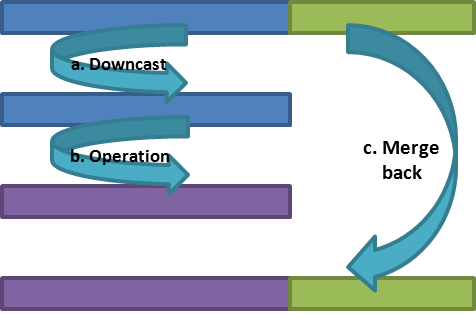
\psfig{file=heap_upcasting.png,height=5cm}} \caption{Coercing references.\label{fig:ref_coerce}}
\end{figure}

We instance the coercion predicate for references to perform a single step of coercion, that is for the case when we have a reference to a memory $tl$ and we want to use it where we expect a memory $Cons\ h\ tl$:
\begin{lstlisting}
class HList tl => Coercible (Ref tl a) (Ref (Cons h tl) a) where
  coerce ref =
    Ref (ST(\(Cons h tl) ->
      let (tl$'$,res) = get ref tl
      in (h $'$Cons$'$ tl$'$, res))
        (\v -> ST(\(Cons h tl) -> 
          let (tl$'$,()) = set ref tl v
          in (h $'$Cons$'$ tl$'$, ())))
  where get (Reference (ST g) _) = g
    set (Reference _ s) = \st -> \v -> 
      let (ST s$'$) = s v
      in s$'$ st
\end{lstlisting}

Now we can finally rewrite the example above to make use of our new coercion operator:
\begin{lstlisting}
ex3 :: ST Nil Unit
ex3 = do+ i <- new 10 :: Ref (New Nil Int) Int
          s <- new "Hello" :: Ref (New (New Nil Int) String) String
          (coerce i) *= (+2)
          s *= (++" World")
          return ())
\end{lstlisting}
